
\documentclass[a4paper,10pt]{article}
\usepackage{listings,color,epsfig,amsmath,url}
\definecolor{codecolor}{rgb}{0.99,0.97,0.94} % color values Red, Green, Blue
\definecolor{commentcolor}{rgb}{0.1,0.5,0.1} % color values Red, Green, Blue
\definecolor{stringcolor}{rgb}{0.3,0.1,0.1} % color values Red, Green, Blue
\newcommand{\Code}[1]{\texttt{#1} }
\newcommand{\code}[1]{\Code{#1} }
\newcommand{\DB}   {\code{{MOOSDB}}}
\newcommand{\MA}   {\code{{MOOSApp}}}
\newcommand{\Ignore}[1]   {}



% Title Page
\title{Logging with \code{pLogger}}
\author{Paul Newman}


\begin{document}
\maketitle

\begin{center}

\epsfig{file=images/moose6.eps,width = 0.2\linewidth}
\end{center}

\section{Logging - \code{pLogger}}
The \code{pLogger} process is intended to record the activities of
a MOOS session. It can be configured to record a fraction of or
every publication of any number of MOOS variables. It is an
essential MOOS tool and is worth its weight in gold in terms of
post-mission analysis, data gathering and post-mission replay.

The configuration of \code{pLogger} is trivial and consists of
multiple lines with the following syntax:
\begin{center}
\code{Log} =  {\it{varname}} @ {\it{period}} $[NOSYNC],[MONITOR]$
\end{center}
where {\it{varname}} is any MOOS variable name and {\it{period}}
is the minimum interval between log entries that will be recorded
for the given variable. For example if
{\it{varname}}=\code{INS\_YAW} and {\it{period}} = 0.2 then even
if the variable is published at 20Hz it will only be recorded at
5Hz. The optional \code{NOSYNC} flag indicates that this variable
should not be recorded in the synchronous logs (see section
\ref{sec:LogTypes}). The optional \code{MONITOR} flag tells \code{pLogger} to send a notification if this variable isn't logged at least every 10 seconds. The notification occurs under the \code{MOOS\_DEBUG} variable. If you are running \code{iRemote} (which subscribes to this variable
automatically) you'll see a warning printed to the screen. This can be pretty useful when runnning
a complicated system and you really do want notification that an important variable isn't being logged (probably because the process producing the variable is kaput in some sense.)

\subsection{Logging Session}

The logger supports the notion of Logging Sessions. For each log session the Logger will create a new directory and place all the logged files within that directory. These are typically (see later sections) an alog file a slog file a system log file, a copy of the mission file (moos file) and if applicable a hoof file (if  \code{pHelm} is running). A new log session can be created by writing the variable \code{LOGGER\_RESTART} to the \code{MOOSDB} or if you are using \code{iRemote} by pressing shift-g.

\subsection{Log File Types}\label{sec:LogTypes}
The logger records data in two file formats - synchronous
(``slog'' extensions) and asynchronous (``alog'' extensions). Both
formats are ASCII text -- they can always be compressed later and
usability is more important than disk space. The two formats are
now discussed.

\subsubsection{Synchronous Log Files}
Synchronous logging makes a table of {\em{numerical}} data. Each
line in the file corresponds to a single time interval. Each
column of the table represents the broad evolution of a given
variable over time. The time between lines (and whether
synchronous logging is even required) is specified with the line
\begin{center}
\code{SyncLog}= {\it{true/false @ period}}
\end{center}
where {\it{period}} is the interval time.

If there has been no change in the numeric variable between
successive time steps then its value is written as \code{NaN}. It
is important to note that synchronous logs do not capture all that
happens - they sample it. Synchronous logs are designed to be used
to swiftly appraise the behaviour of a MOOS community by examining
numeric data in a tool such as Matlab or a spreadsheet. The
\code{MOOSData} Matlab script reads in these files and with a
single mouse click can display the time evolution of any logged
variable.


\subsubsection{Asynchronous Log Files}
Asynchronous logging is thorough. The mechanism is designed to be
able to record {\em{every}} delta to the MOOSDB. The use of the
period variable allows the mission designer to back off from this
ultimate limit and record variables at a maximum frequency. The
key properties of asynchronous can be enumerated as follows:
\begin{enumerate}
\item Records both string and numeric data
\item Records data in a list format - one notification per line
\item Entries only made when variable is written
\end{enumerate}
Asynchronous log files are designed to be used with a playback
tool (for example \code{uPlayback} or other purpose-built
executable). Although the handling of strings and numeric data
adds a slight overhead to such a program's complexity the utility
gain from being able to slow, stop and accelerate time during a
post-mission replay/reprocessing session is simply massive.


\subsubsection{Mission Backup}
Simply having the {\it{alog}} and {\it{slog}} files is not enough
to evaluate the mission. One also needs the things that
{\em{caused}} the data to be recorded, namely the *.moos Mission
file and the *.hoof file (if Task redirection was used). To this
end the \code{pLogger} process takes a copy of these files and
places them (name appended with a time stamp if desired) within
the logging directory. The files extensions are renamed to
{\it{*.\_moos}} and {\it{*.\_hoof}} respectively.




\section{Replay -- \code{uPB}}
There is a FLTK-based, cross platform GUI application that can
load in {\it{alog}} files and replay them into a MOOS community as
though the originators of the data were really running and issuing
notifications. A typical use of this application is to ``fake''
the presence of sensor processes when reprocessing sensor data and
tuning navigation filters. Alternatively it can be used in pure
replay mode perhaps to render a movie of the recorded mission. The
GUI allows the selection of which processes are ``faked''. Only
data recorded from those applications will be replayed from the
log files.  There is a single class that encapsulates all the
replay functionality - \code{CMOOSPlayback}. The GUI simply hooks
into the methods exported by this class. The GUI is almost self
documenting - start it up and hold the mouse over various buttons.

\begin{figure}
\center 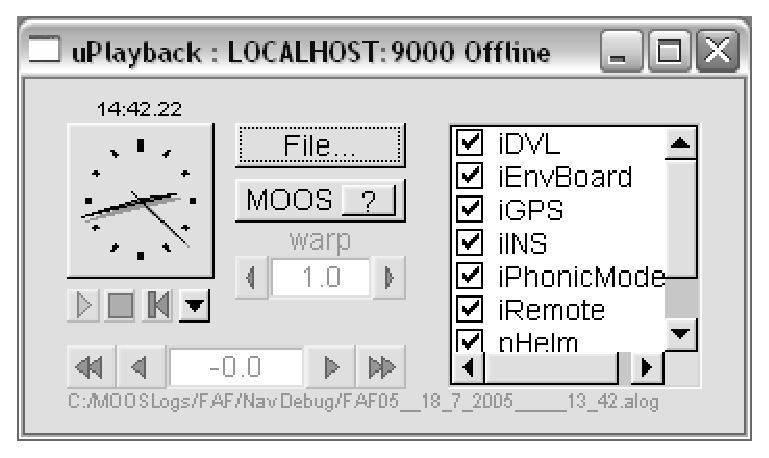
\epsfig{file=images/uPB.eps,width = 0.8\linewidth} \caption{A
screen shot of \code{uPB} - a cross platform ``alog'' playback
tool}
\end{figure}

A client process can control the replay of MOOS messages by
writing to the \code{PLAYBACK\_CHOKE} variable add writing a valid
time in the numeric message field. The Playback executable will
not play more than a few seconds past this value before waiting
for a new value to be written. In this way  it is possible to
debug (halt inspect and compile-in-place etc) at source level a
client application using replayed data without having the playback
rush on ahead during periods of thought or code-stepping.

\end{document} 